% !TEX root = ../main.tex

% 报告主体


%---------------------------------------------------------------------
% 实验
\clearpage
\ysySection{实验}

\subsection{测试模块的搭建与校准}

在开展纠缠态特性测试之前，为确保实验精度与重复性，我们首先完成了测试模块的搭建与校准工作。该工作主要包括偏振相关光学器件的光轴校准以及整体光路的搭建与调试。

偏振器件的光轴精确对准对于后续的偏振投影测量至关重要。我们采用标准偏振态光源，逐一校准各偏振片与偏振分束器的光轴方向。该步骤由丁侯凯与戴鹏辉负责完成，具体的校准结果列于\cref{tab1}。

\begin{table}[!ht]
	\centering
	\resizebox{\textwidth}{!}{\begin{tabular}{|c|c|c|c|c|c|c|c|}
		\hline
		测试器件:PP-A & 极值点功率 & 角度（°） & H投射方向 & 测试器件:PP-B & 极值点功率 & 角度（°） & H投射方向 \\ \hline
		入射光功率（mW） & 18.000 & 237 & 59° & 入射光功率（mW） & 18.700 & 89 & 89° \\ \hline
		~ & 0.056 & 330 & ~ & ~ & 0.015 & 182 & ~ \\ \hline
		~ & 18.200 & 59 & ~ & ~ & 18.600 & 272 & ~ \\ \hline
		~ & 0.056 & 149 & ~ & ~ & 0.015 & 0 & ~ \\ \hline
		测试器件:QWP-A & 极值点功率 & 角度（°） & 光轴角度 & 测试器件:PP-B & 极值点功率 & 角度（°） & 光轴角度 \\ \hline
		入射光功率（mW） & 13.320 & 20 & 20° & 入射光功率（mW） & 12.990 & 75 & 344° \\ \hline
		~ & 6.790 & 65 & ~ & ~ & 6.520 & 119 & ~ \\ \hline
		~ & 13.330 & 111 & ~ & ~ & 12.970 & 163 & ~ \\ \hline
		~ & 6.730 & 153 & ~ & ~ & 6.720 & 209 & ~ \\ \hline
	\end{tabular}
}
	\caption{偏振片和波片角度校准数据}
	\label{tab1}
\end{table}

随后，我们搭建并调试了测试模块的完整光路系统。该过程主要由戴鹏辉和丁侯凯完成，杨舒云承担部分辅助工作。最终构建完成的测试模块光路如\cref{fig:apl25experimentalopticalpathdiagram}所示，涵盖了信号与闲置光子路径的导引、投影测量器件的布置以及与计数模块的接口连接。

\begin{figure}[h!]
	\centering
	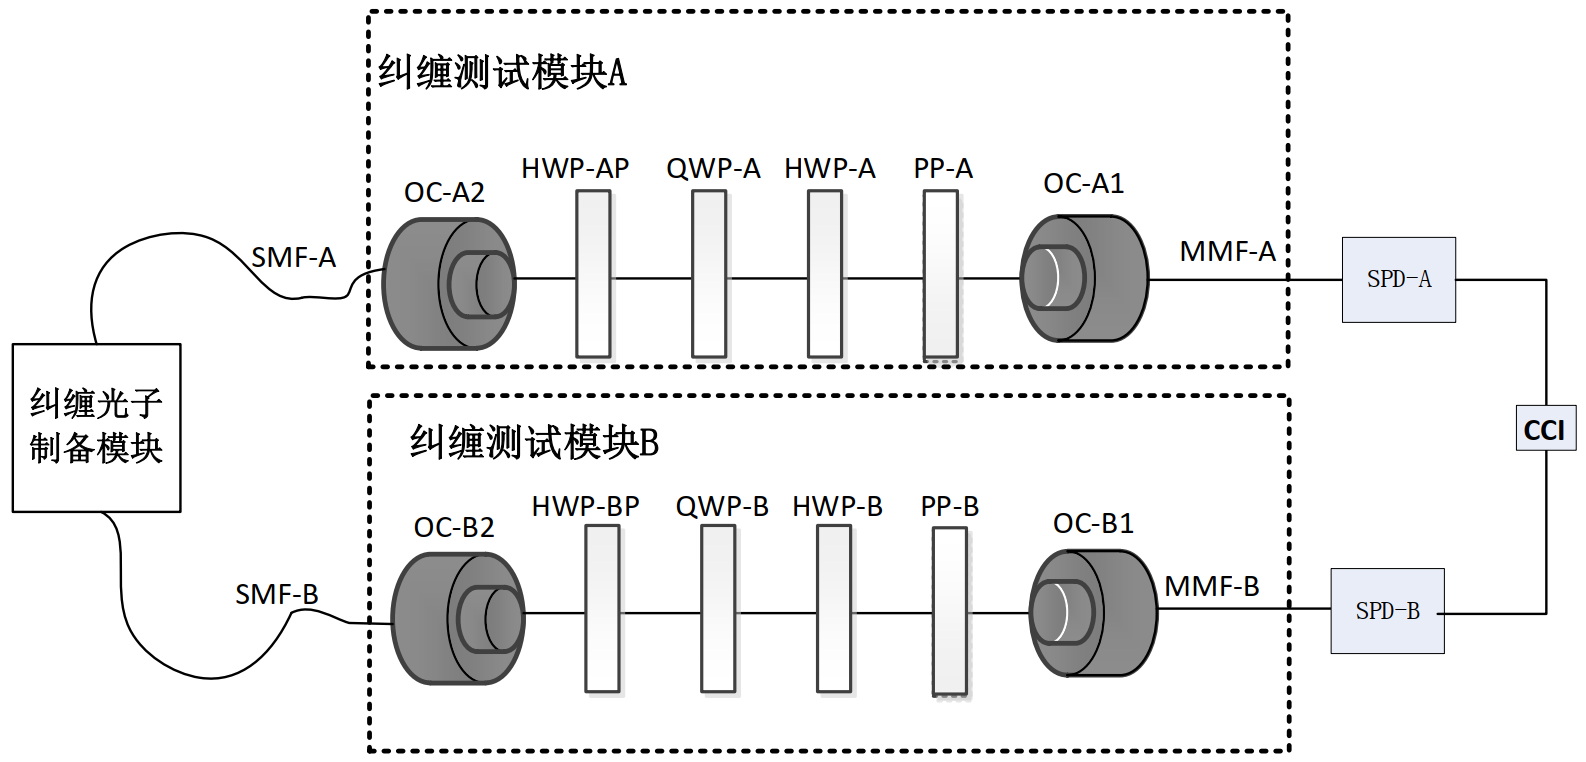
\includegraphics[width=0.9\linewidth]{images/apl2_5_experimental_optical_path_diagram}
	\caption{测试模块的完整光路系统（来自讲义）}
	\label{fig:apl25experimentalopticalpathdiagram}
\end{figure}

至此，实验装置的测试部分已全面搭建完毕，并完成必要的校准工作，为后续的纠缠态验证实验奠定了良好的基础。

\subsection{纠缠特性测试}

我们对纠缠态特性的测试主要包含纠缠亮度和对比度测量、保真度测量以及CHSH 游戏。

\subsubsection{纠缠亮度和对比度测量}
为了评估实验系统产生双光子纠缠态的能力及其质量，我们对纠缠态的亮度和偏振基下的对比度进行了系统测量。实验中使用两个纠缠测试模块，分别标记为 A 和 B。每个模块均配置有一组半波片（HWP-A, HWP-B）与四分之一波片（QWP-A, QWP-B）。具体测量步骤如下：

首先，将 HWP-A 与 HWP-B 均调至 0°，同时将 QWP-A 与 QWP-B 也设定在 0°位置。此时系统处于 $\ket{H}\ket{H}$ 基态的投影设置，记录符合计数仪（Coincidence Counting Instrument, CCI）在积分时间为 10 s 下的符合计数，记为 $C_1$。

随后，将 HWP-A 和 HWP-B 同时旋转至 -45°，对应于 $\ket{V}\ket{V}$ 投影设置，记录符合计数 $C_2$。

接下来，将 HWP-A 从 -45°旋转回 0°，保持 HWP-B 在 -45°，此时对应的符合计数记为 $C_3$。据此可计算单位泵浦光功率下的系统纠缠亮度 $L$，定义为：
\[
L = \frac{C_1 + C_2 - 2C_3}{P}
\]
其中 $P$ 表示入射泵浦光功率。

在对比度测量中，我们首先将 HWP-A 和 HWP-B 同时设定为 -22.5°，对应于 $D/A$ 基的相干投影（即 $\ket{+}\ket{+}$），记录符合计数 $C_4$。随后，将 HWP-A 旋转至 +22.5°，保持 HWP-B 为 -22.5°，记录符合计数 $C_5$。

利用符合计数数据，可分别计算系统在 $H/V$ 基和 $+/-$ 基下的纠缠对比度，定义如下：
\begin{itemize}
	\item $H/V$ 基对比度：
	\[
	V_{HV} = \frac{C_1 - C_3}{C_1 + C_3}
	\]
	
	\item $+/-$ 基对比度：
	\[
	V_{+-} = \frac{C_4 - C_5}{C_4 + C_5}
	\]
\end{itemize}

测量主要由杨舒云、戴鹏辉完成，丁侯凯记录数据，结果如\cref{tab2}所示。

\begin{table}[h!]
	\centering
	\begin{tabular}{|c|c|c|c|c|c|}
		\hline
		\textbf{通道名称} & \textbf{C1} & \textbf{C2} & \textbf{C3} & \textbf{C4} & \textbf{C5} \\ \hline
		\textbf{通道1} & 29976 & 29210 & 26068 & 28090 & 27499 \\ \hline
		\textbf{通道2} & 13532 & 12700 & 13487 & 13060 & 12539 \\ \hline
		\textbf{OUT} & 1936 & 1376 & 63 & 230 & 1403 \\ \hline
	\end{tabular}
	\caption{纠缠亮度和对比度测量实验数据}
	\label{tab2}
\end{table}

由此计算得到：
$$ V_{HV} = 93.70\% $$
$$ V_{+-} = 71.83 \% $$

$H/V$ 基下的对比度接近理想最大值，表明系统在直线偏振基底中具有良好的干涉可见度，光学器件的校准精度与双光子干涉稳定性较高。与此同时，$+/-$ 基下对比度略低，可能来源于以下因素：光学路径中存在轻微的相位漂移或器件偏差，影响了两个路径之间的相干性；波片的实际相位延迟值与标称值存在偏差，尤其在 $+/-$ 基的干涉测量中更为敏感；计数器或单光子探测器的探测效率非均匀，可能对部分偏振态存在系统性偏倚。

尽管 $+/-$ 基下的对比度相对较低，但其仍明显高于经典系统的典型阈值，说明该实验系统确实制备出了具有非经典相关性的纠缠态。结合两个基底的高对比度表现，可以初步确认所制备态在偏振自由度上具备明显的纠缠特征，为进一步开展量子态层析重构与 Bell 不等式验证实验提供了坚实的基础。

\subsubsection{保真度测量}
为了进一步定量表征实验所制备纠缠态与理想 Bell 态之间的一致性，我们对其进行了保真度测量。该测量基于前述 Bell 不等式测试所用的角度设置，并通过密度矩阵重构获取。

实验过程中，首先根据理论预设的 Bell 不等式测试方案确定各测量基下的半波片旋转角度，并严格按照表格要求调节 HWP-A 与 HWP-B 的偏振角。符合计数数据由符合计数仪（CCI）记录，数据采集工作由杨舒云与戴鹏辉完成，数据记录由丁侯凯与黄罗琳负责。全部测量结果如\cref{tab3}所示。

\begin{table}[h!]
	\centering
	\begin{tabular}{|l|l|l|l|l|l|}
		\hline
		测量基 & HWP\_A & QWP\_A & HWP\_B & QWP\_B & 符合仪计数 \\ \hline
		HH & 306.00 & 111.00 & 67.00 & 254.00 & 1800 \\ \hline
		HV & 306.00 & 111.00 & 112.00 & 254.00 & 10 \\ \hline
		HL & 306.00 & 111.00 & 89.50 & 254.00 & 800 \\ \hline
		HD & 306.00 & 111.00 & 89.50 & 299.00 & 1050 \\ \hline
		VD & 351.00 & 111.00 & 89.50 & 299.00 & 475 \\ \hline
		VL & 351.00 & 111.00 & 89.50 & 254.00 & 725 \\ \hline
		VH & 351.00 & 111.00 & 67.00 & 254.00 & 15 \\ \hline
		VV & 351.00 & 111.00 & 112.00 & 254.00 & 1150 \\ \hline
		LV & 328.50 & 111.00 & 112.00 & 254.00 & 600 \\ \hline
		LH & 328.50 & 111.00 & 67.00 & 254.00 & 875 \\ \hline
		LL & 328.50 & 111.00 & 89.50 & 254.00 & 100 \\ \hline
		LD & 328.50 & 111.00 & 89.50 & 299.00 & 600 \\ \hline
		DD & 328.50 & 156.00 & 89.50 & 299.00 & 1300 \\ \hline
		DL & 328.50 & 156.00 & 89.50 & 254.00 & 500 \\ \hline
		DH & 328.50 & 156.00 & 67.00 & 254.00 & 750 \\ \hline
		DV & 328.50 & 156.00 & 112.00 & 254.00 & 750 \\ \hline
	\end{tabular}
	\caption{保真度测量实验数据}
	\label{tab3}
\end{table}

随后，采用计算机程序对采集到的符合计数数据进行密度矩阵重构与保真度计算。该部分工作由黄罗琳与戴鹏辉协作完成。实验结果如下：

对于理想的 $\ket{\Phi^+} = \frac{1}{\sqrt{2}}(\ket{HH} + \ket{VV})$ 态，即 +Bell 态，计算得两组保真度分别为：
\[
F_1 = 0.9275,\quad F_2 = 0.9151,
\]
平均保真度约为 0.9213 ，表明制备态与目标 Bell 态之间具有较高的一致性，纠缠质量良好。总符合计数为 $E = 2975$。

所重构的密度矩阵如下：

密度矩阵实部：
\[
Re[\rho]=\begin{bmatrix}
	0.5974 & 0.0442 & -0.0538 & 0.4208 \\
	0.0442 & 0.0055 & -0.0037 & 0.0423 \\
	-0.0538 & -0.0037 & 0.0060 & -0.0391 \\
	0.4208 & 0.0423 & -0.0391 & 0.3911 \\
\end{bmatrix}
\]

密度矩阵虚部：
\[
Im[\rho]=\begin{bmatrix}
	0 & -0.0302 & -0.0132 & -0.1303 \\
	0.0302 & 0 & -0.0044 & 0.0128 \\
	0.0132 & 0.0044 & 0 & 0.0244 \\
	0.1303 & -0.0128 & -0.0244 & 0 \\
\end{bmatrix}
\]

同时，我们对其与 -Bell 态 $\ket{\Phi^-} = \frac{1}{\sqrt{2}}(\ket{HH} - \ket{VV})$ 之间的保真度也进行了计算，结果远低，仅为：
\[
F_1 = 0.1065,\quad F_2 = 0.0734,
\]
表明实验所得态与 -Bell 态之间的一致性极低，进一步印证了本次实验系统优先制备的是 $\ket{\Phi^+}$ 态。

事实上，我们对实验室提供的保真度计算程序的计算结果在一定程度上保持怀疑，基于这一原因我们自行探究并尝试开发了用于本实验保真度计算的基于iMLE方法的量子态断层扫描密度矩阵重构方案并得到了不一样的结果，具体内容详见分析与讨论部分。

\subsubsection{CHSH游戏}
为验证实验制备态在量子非局域性测试中的有效性，我们引入 CHSH 游戏框架对系统进行测试。CHSH（Clauser-Horne-Shimony-Holt）游戏是一种量子非局域性验证方式，其核心思想是通过一系列随机选择的局域测量设置，检验系统是否能够超越经典局域隐变量理论所允许的最大胜率上限。

本实验中，采用波片与偏振片组成的偏振基矢选择装置，其中偏振片固定，半波片作为唯一可调元件，用于实现不同测量基的选择。因此，实验的主要操作部件为测试模块中的 HWP-A 与 HWP-B。

由于进行本实验时，我们更换了操作台，新的光学元件标定数据如\cref{tab4}所示。

\begin{table}[h!]
	\centering
	\begin{tabular}{|c|c|c|c|}
		\hline
		\textbf{HWP-A} & \textbf{QWP-A} & \textbf{HWP-B} & \textbf{QWP-B} \\ \hline
		315° & 260° & 226° & 215° \\ \hline
	\end{tabular}
	\caption{CHSH游戏实验台光学元件标定数据}
	\label{tab4}
\end{table}

实验步骤如下：
\begin{enumerate}
	\item 根据 CHSH 游戏的测量方案，构造测量基与输入输出对应关系，并计算 HWP-A 和 HWP-B 所需设置的旋转角度；
	\item 按照数据表格中指定的角度，依次调整两模块中的半波片，并在每一组输入 $(x, y)$ 下记录对应输出 $(a, b)$ 的符合计数值；
	\item 汇总全部测量数据，根据标准 CHSH 游戏胜率定义，计算系统的实际平均胜率。
\end{enumerate}

上述实验操作由黄罗琳与戴鹏辉完成，数据统计结果如\cref{tab5}所示。

\begin{table}[h!]
	\centering
	\resizebox{\textwidth}{!}{\begin{tabular}{|c|c|c|c|c|c|c|c|c|}
		\hline
		\textbf{裁判问题} & \textbf{态操作对应的偏振旋转} & \textbf{测量基} & \textbf{HWP-A} & \textbf{} & \textbf{HWP-B} & \textbf{} & \textbf{符合计数} & \textbf{胜率} \\ \hline
		~ & ~ & ~ & 理论值 & 实际值 & 理论值 & 实际值 & ~ & ~ \\ \hline
		X = 0 &  θA0 = 0 & HH & 0 & 315 & 11.25 & 237.25 & 1160 & 77.92\% \\ \hline
		Y = 0 & θB0 = 22.5° & HV & 0 & 315 & -33.75 & 192.25 & 280 & ~ \\ \hline
		~ & ~ & VH & -45 & 270 & 11.25 & 237.25 & 380 & ~ \\ \hline
		~ & ~ & VV & -45 & 270 & -33.75 & 192.25 & 1170 & ~ \\ \hline
		X = 0 &  θA0 = 0 & HH & 0 & 315 & -11.25 & 214.75 & 1180 & 87.21\% \\ \hline
		Y = 1 & θB1 = -22.5° & HV & 0 & 315 & -56.25 & 169.75 & 200 & ~ \\ \hline
		~ & ~ & VH & -45 & 270 & -11.25 & 214.75 & 190 & ~ \\ \hline
		~ & ~ & VV & -45 & 270 & -56.25 & 169.75 & 1480 & ~ \\ \hline
		X = 1 &  θA1 = 45° & HH & 22.5 & 337.5 & 11.25 & 237.25 & 1150 & 76.09\% \\ \hline
		Y = 0 & θB0 = 22.5° & HV & 22.5 & 337.5 & -33.75 & 192.25 & 320 & ~ \\ \hline
		~ & ~ & VH & -22.5 & 292.5 & 11.25 & 237.25 & 390 & ~ \\ \hline
		~ & ~ & VV & -22.5 & 292.5 & -33.75 & 192.25 & 1110 & ~ \\ \hline
		X = 1 &  θA1 = 45° & HH & 22.5 & 337.5 & -11.25 & 214.75 & 470 & 62.82\% \\ \hline
		Y = 1 & θB1 = -22.5° & HV & 22.5 & 337.5 & -56.25 & 169.75 & 1080 & ~ \\ \hline
		~ & ~ & VH & -22.5 & 292.5 & -11.25 & 214.75 & 880 & ~ \\ \hline
		~ & ~ & VV & -22.5 & 292.5 & -56.25 & 169.75 & 690 & ~ \\ \hline
	\end{tabular}
}
\caption{CHSH 游戏测量数据}
\label{tab5}
\end{table}

实验得到的 CHSH 游戏平均胜率为：
\[
P_\text{win} = 76.01\%.
\]

该结果高于经典局域理论所允许的最大胜率 75\%，但偏离理想量子理论上限 $P_\text{win}^\text{quantum} = \cos^2\left(\frac{\pi}{8}\right) \approx 85.36\%$ 较远。实验细节中可能存在的系统误差或相干性损失对结果造成了一定影响，具体讨论详见“分析与讨论”部分。

该测量结果从统计意义上支持了实验所制备纠缠态具备一定的非局域性表现，但同时也反映出实验系统在光学对准、波片误差或计数稳定性等方面仍存在改进空间。

%---------------------------------------------------------------------
% 分析与讨论
\ysySection{分析与讨论}

\subsection{基于iMLE方法的量子态断层扫描与保真度计算}

\subsubsection{保真度}
\textbf{保真度（Fidelity）}是用来衡量两个量子态相似程度的指标，数值范围在 \([0,1]\) 之间，\( F = 1 \) 表示两个量子态完全相同，\( F = 0 \) 表示它们完全不同。

如果两个量子态分别由密度矩阵 \( \rho \) 和 \( \sigma \) 描述，保真度的定义（注意另一种常见的定义为本定义的平方）为：
\[
F(\rho, \sigma) =  \text{Tr} \sqrt{\sqrt{\rho} \sigma \sqrt{\rho}} 
\]
其中，\( \text{Tr} \) 表示矩阵的迹（trace）；\( \sqrt{\rho} \) 表示对密度矩阵 \( \rho \) 取平方根。

对于本实验来说，我们可以认为我们要制备的是Bell态$|\Phi^+\rangle = \frac{1}{\sqrt{2}} (|00\rangle + |11\rangle)$，它的密度矩阵为：
\[
\rho_{\Phi^+} = |\Phi^+\rangle \langle \Phi^+|
\]
\[
= \frac{1}{2} (|00\rangle + |11\rangle)(\langle 00| + \langle 11|)
\]
\[
= \frac{1}{2} \begin{bmatrix} 
	1 & 0 & 0 & 1 \\ 
	0 & 0 & 0 & 0 \\ 
	0 & 0 & 0 & 0 \\ 
	1 & 0 & 0 & 1
\end{bmatrix}
\]

因此我们需要从测量结果中获得我们制备的态的$\rho$，这就要用到量子态断层扫描。

\subsubsection{量子态断层扫描}
\textbf{量子态断层扫描（Quantum State Tomography, QST）}是一种实验技术，用于重构未知的量子态，即测量和推断密度矩阵 \( \rho \) 的方法。在量子信息处理中，QST 是一个重要的工具，广泛用于量子计算、量子通信和纠缠态的实验研究。由于量子测量通常会破坏态本身，并且单次测量只能提供有限的信息，因此无法直接读取量子态，而需要通过一系列不同的测量来重构整个密度矩阵 \( \rho \)。一个 \( d \) 维的量子态（即 \( n = \log_2 d \) 量子比特）可以用 \( d^2 - 1 \) 个独立的参数表示，因此 QST 需要足够多的独立测量来确定这些参数。  

QST 主要依赖于选取合适的测量基进行实验测量，并利用这些测量数据重构密度矩阵。常见的测量基包括泡利算符基（Pauli Basis），即测量泡利矩阵 \( \sigma_x, \sigma_y, \sigma_z \) 的期望值：  
\[
\sigma_x = \begin{bmatrix} 0 & 1 \\ 1 & 0 \end{bmatrix}, \quad
\sigma_y = \begin{bmatrix} 0 & -i \\ i & 0 \end{bmatrix}, \quad
\sigma_z = \begin{bmatrix} 1 & 0 \\ 0 & -1 \end{bmatrix}
\]  
此外，也可以使用 SIC-POVM（对称、信息完整的正定测量）等超完备测量方法以减少统计误差并提高重构精度。在泡利基下，密度矩阵可以表示为  
\[
\rho = \frac{1}{2^n} \sum_{i_1, i_2, ..., i_n} c_{i_1 i_2 ... i_n} \, \sigma_{i_1} \otimes \sigma_{i_2} \otimes ... \otimes \sigma_{i_n}
\]  
其中，\( c_{i_1 i_2 ... i_n} \) 是泡利矩阵的期望值，由实验测量得到：  
\[
c_{i_1 i_2 ... i_n} = \text{Tr}(\rho \cdot (\sigma_{i_1} \otimes \sigma_{i_2} \otimes ... \otimes \sigma_{i_n}))
\]  
通过这些测量结果，我们可以完全重构密度矩阵。  

QST 的实验过程通常包括以下几个步骤：首先制备未知的量子态 \( \rho \)，然后选择一组测量基（如泡利算符基），接着进行大量次测量，每次对量子态进行投影测量，并统计测量结果的频率，最后通过最大似然估计（Maximum Likelihood Estimation, MLE）或贝叶斯估计（Bayesian Estimation）重构密度矩阵。例如，对于单量子比特的情况，其密度矩阵可以表示为  
\[
\rho = \frac{1}{2} (I + a_x \sigma_x + a_y \sigma_y + a_z \sigma_z)
\]  
其中，\( a_x, a_y, a_z \) 是泡利矩阵的期望值：  
\[
a_x = \text{Tr}(\rho \sigma_x), \quad a_y = \text{Tr}(\rho \sigma_y), \quad a_z = \text{Tr}(\rho \sigma_z)
\]  
通过实验测量这些期望值后，即可求得密度矩阵。  

\subsubsection{iMLE方法、结果与后续展望}
为进一步全面表征双光子纠缠态的密度矩阵结构，本实验基于最大似然估计（Maximum Likelihood Estimation, MLE）方法进行量子态断层扫描（Quantum State Tomography）。其中，\textbf{初始密度矩阵采用线性反演（linear inversion）方式获得}，并作为 iMLE 算法的初始输入，最终得到满足物理约束（Hermiticity、正定性与归一性）的密度矩阵。

\begin{itemize}
	\item 实验中采用 $\{H, V, D, L\}$ 四组偏振态作为单比特测量基，其中，$H = \ket{0}$，$V = \ket{1}$，$D = \frac{1}{\sqrt{2}}(\ket{0} + \ket{1})$以及$L = \frac{1}{\sqrt{2}}(\ket{0} + i\ket{1})$。
	
	构造出的 16 个双比特投影测量算符 $\{P_{AB} = \ket{A}\bra{A} \otimes \ket{B}\bra{B}\}$，覆盖了 $HH, HV, \dots, DV$ 全部基对，分别对应一组符合计数实验数据，详见测量统计：
	\[
	\text{总符合计数} = 2975，\quad \text{归一化后用于断层重构的概率矢量 } \{p_i\}
	\]
	
	通过构造线性方程组 $p_i = \operatorname{Tr}(P_i \rho)$ 并利用 Moore–Penrose 伪逆求解得到初始密度矩阵 $\rho_{\text{linear}}$。该矩阵随后进行物理性修正（Hermiticity、谱截断与归一化），以满足基本的量子态约束。最终重构密度矩阵为：
	\[
	\rho_{\text{linear}} =
	\begin{bmatrix}
		0.577 & 0.041 & -0.076 & 0.434 \\
		0.041 & 0.006 & 0.001 & 0.025 \\
		-0.076 & 0.001 & 0.021 & -0.068 \\
		0.434 & 0.025 & -0.068 & 0.396 \\
	\end{bmatrix}
	\]
	
	与理想 Bell 态 $\ket{\Phi^+} = \frac{1}{\sqrt{2}}(\ket{HH} + \ket{VV})$ 的保真度为：
	\[
	F_{\text{linear}} = 0.9592
	\]
	显示出非常接近目标态的纠缠特性。
	
	具体而言，我们首先以 np.outer 构造 $\ket{A}\bra{A} \otimes \ket{B}\bra{B}$ 的双比特测量投影算符，并整理为列表 measurement\_ops。每个测量基对应的实验归一化频率则整理为 measured\_probs。利用这些信息，我们建立了如下形式的线性方程组：
	\[
	\mathbf{p} = A \cdot \text{vec}(\rho),
	\]
	其中 $A$ 是由测量算符 $\{M_i\}$ 的转置张量积构成的矩阵，$\text{vec}(\rho)$ 是将密度矩阵按行展平后的向量。通过 np.linalg.pinv 实现广义逆矩阵求解，得到线性反演的 $\rho_{\text{linear}}$。
	
	\item 进一步采用\textbf{迭代最大似然估计算法（iMLE）}对密度矩阵进行优化重构，具体迭代过程参考文献 \cref{ref:2}所提出的框架。简言之，在线性反演的基础上，我们进一步实现了经典的迭代最大似然估计算法（iMLE），其核心过程是反复构造权重矩阵 $Q$ 并迭代更新 $\rho$，代码结构参考文献 [2] 中提出的方案。实现中我们加入了以下数值优化策略：为避免除以零，对理论概率 $p_i$ 设置下限；保证每一步结果满足 Hermiticity 与正定性（通过特征值截断）；使用 np.linalg.eigh 实现谱分解与重构。最后，通过 QuTiP 提供的 fidelity() 函数，我们分别计算了 $\rho_{\text{linear}}$ 与 $\rho_{\text{MLE}}$ 相对于理想 Bell 态的保真度。
	
	最终获得的密度矩阵为：
	\[
	\rho_{\text{MLE}} =
	\begin{bmatrix}
		0.433 & 0.210 - 0.139i & 0.192 - 0.131i & 0.130 - 0.334i \\
		0.210 + 0.139i & 0.146 & 0.135 - 0.002i & 0.170 - 0.120i \\
		0.192 + 0.131i & 0.135 + 0.002i & 0.125 & 0.159 - 0.109i \\
		0.130 + 0.334i & 0.170 + 0.120i & 0.159 + 0.109i & 0.296 \\
	\end{bmatrix}
	\]
	
	计算其与目标 Bell 态的保真度得：
	\[
	F_{\text{MLE}} = 0.7030
	\]
	
	这一结果低于线性反演所得保真度，也\textbf{显著低于实验室程序计算}所得 $F \approx 0.9213$。这表明在本实验数据及选择的测量基下，\textbf{iMLE 方法的收敛质量较差}，可能由于：投影测量设置未能充分涵盖高灵敏方向（参见 \cref{ref:5}）；观测概率分布中存在统计波动，影响 MLE 收敛；本实验中所用 iMLE 算法迭代方式为最基础型，未做稀释（dilution）或超加速（superfast）优化。
	
	\item 针对当前 iMLE 收敛性不足的问题，可考虑采用以下方法进一步优化密度矩阵重构结果：引入稀释 MLE（diluted MLE）算法 \cref{ref:3}，提升稳定性；使用 \textbf{Superfast MLE 算法} \cref{ref:4}，加速收敛并避免陷入局部最优；利用\textbf{神经网络生成对抗网络（CGAN）方法} \cref{ref:5}，实现数据驱动的稳健态重构。
	
	此外，在文献 \cref{ref:5} 提供的 GitHub 实例中展示了：即使在无噪声的模拟数据下，iMLE 方法仍可能失败，而神经网络方法则成功恢复目标态。这表明数据与测量基的选择对 iMLE 的性能具有高度敏感性。
\end{itemize}

\subsection{CHSH 游戏结果分析}

\subsubsection{对测试模块光学元件作用的探讨}
根据测试模块光路\cref{fig:apl25experimentalopticalpathdiagram}，我们以一路为例子，具体探讨光学元件HWP-AP、QWP-A、HWP-A、PP-A的作用。
\begin{itemize}
	\item \textbf{HWP-AP：通道偏振补偿波片}
	
	HWP-AP 是一块固定角度的半波片，通常用于补偿光纤耦合和自由空间耦合过程引入的偏振旋转或相位延迟。由于光纤具有一定双折射性，输出偏振态可能偏离期望的 $H/V$ 基，HWP-AP 的主要任务是将光子偏振重新调整至标准线性基底，使后续的波片操作具有良好的基准态。
	
	在数学上，半波片对于偏振态 $\ket{\psi}$ 的作用可以表示为：
	\[
	U_{\text{HWP}}(\theta) = \cos(2\theta) \sigma_x + \sin(2\theta) \sigma_y,
	\]
	其中 $\theta$ 为波片光轴相对于水平轴的夹角，$\sigma_x$ 和 $\sigma_y$ 是 Pauli 矩阵。
	
	HWP-AP 通常固定设置为 0° 或 -22.5°，以实现特定基态的标准化。
	
	\item \textbf{QWP-A：圆偏振到线偏振的转换器}
	
	QWP-A 是测试模块中用于引入圆偏振基（$L/R$）信息的关键元件。在量子态断层扫描中，为实现对不同基下的投影测量，必须引入非线性偏振方向（如 $\ket{L} = \frac{1}{\sqrt{2}}(\ket{H} + i\ket{V})$），四分之一波片的作用正是提供该自由度。
	
	QWP 的 Jones 矩阵如下：
	\[
	U_{\text{QWP}}(\theta) = \begin{bmatrix}
		\cos^2\theta + i\sin^2\theta & (1 - i)\cos\theta\sin\theta \\
		(1 - i)\cos\theta\sin\theta & \sin^2\theta + i\cos^2\theta
	\end{bmatrix}.
	\]
	
	QWP-A 可将 $\ket{L}$ 转换为 $\ket{H}$ 或 $\ket{V}$，使系统仍可使用固定偏振片实现圆偏振投影测量。通过旋转 QWP-A 与后续 HWP-A 的角度组合，可以实现对 $H/V$、$D/A$、$L/R$ 三组正交基的全面投影。
	
	\item \textbf{HWP-A：主控投影角设定器}
	
	HWP-A 是本实验测试模块中最核心的控制元件，其旋转角直接决定测量基的选择。通过设定特定角度（如 0°、22.5°、-22.5°、45° 等），可以实现：
	\begin{itemize}
		\item 在 $H/V$ 基下：测量 $\ket{H}$ 或 $\ket{V}$；
		\item 在 $D/A$ 基下：测量 $\ket{+} = \frac{1}{\sqrt{2}}(\ket{H} + \ket{V})$ 或 $\ket{-}$；
		\item 在 $L/R$ 基下：配合 QWP 实现 $\ket{L}$、$\ket{R}$ 投影。
	\end{itemize}
	在 CHSH 游戏和 Bell 不等式测试中，HWP-A 的具体旋转角构成了不同测量设置 $A_0, A_1$，是非局域性验证的关键操作量。
	
	\item \textbf{PP-A（Polarizer）：偏振投影器}
	
	PP-A 是固定的偏振片，设置为 $H$ 或 $V$ 的透射方向。在实验中，其作用是将前面一系列波片调控后的偏振态进行最终投影选择，相当于执行 $\ket{H}\bra{H}$ 或 $\ket{V}\bra{V}$ 的物理测量。
	
	由于偏振片本身无法调节，因此实验中所有的测量基变换都由前置的 HWP/QWP 系统完成，偏振片作为统一终端执行。
	
\end{itemize}

\subsubsection{对实验结果的探讨与分析}
\begin{itemize}
	\item 从原理上回顾，CHSH 游戏中，Alice 和 Bob 接收二进制输入 $x, y \in \{0, 1\}$，输出 $a, b \in \{0,1\}$，若满足：
	\[
	a \oplus b = x \cdot y,
	\]
	则称为“赢得”该轮游戏。
	
	对于制备在理想的 Bell 态 $\ket{\Phi^+} = \frac{1}{\sqrt{2}}(\ket{HH} + \ket{VV})$ 上的系统，若选择测量角度为：
	- $A_0 = 0^\circ,\quad A_1 = 45^\circ$
	- $B_0 = 22.5^\circ,\quad B_1 = -22.5^\circ$
	
	则理论预测的最大胜率为：
	\[
	P_{\text{win}}^{\text{quantum}} = \frac{2 + \sqrt{2}}{4} \approx 85.36\%.
	\]
	
	测量对应的偏振投影方向为：
	\[
	\begin{aligned}
		A_0 &\rightarrow \ket{0},\quad A_1 \rightarrow \frac{\ket{0} + \ket{1}}{\sqrt{2}} \\
		B_0 &\rightarrow \frac{\ket{0} + \ket{1}}{\sqrt{2}},\quad B_1 \rightarrow \frac{\ket{0} - \ket{1}}{\sqrt{2}} \\
	\end{aligned}
	\]
	
	上述映射通过调整 HWP 的角度 $\theta$ 实现投影到 $\cos(2\theta)\ket{H} + \sin(2\theta)\ket{V}$ 上。
	
	从\cref{tab5}可见，HWP-A 与 HWP-B 的实际角度偏离理论角度显著（最大达 $\sim$ 56°），例如理应设置 $-33.75^\circ$ 的 HWP-B 实际角度为 $192.25^\circ$。由于半波片的转换规则为旋转 $2\theta$，这种偏差导致投影态与理论基向量的夹角产生非线性误差，测量基之间的干涉条纹对比度下降，直接影响各投影下的符合概率。
	
	例如，在 $(x,y)=(1,1)$ 的任务中，HH 项计数为 470，远低于其它输入下的 HH 项，这也正是其胜率最低的原因。理论上，该任务对应的赢取概率应与其它输入相近（约 85\%），但由于该配置对应的投影角偏差最大（超过 20°），结果导致量子关联无法有效展示。
	
	以 $(x,y) = (1,1)$ 为例，其四个输出 $(a,b)$ 对应计数如下：$(a,b)=(0,0)$：HH = 470 → 这是“失败”输出；其余为“成功”输出（HV, VH, VV）总计 = 1080 + 880 + 690 = 2650。
	
	胜率计算：
	\[
	P_{\text{win}}^{(x=1,y=1)} = \frac{2650}{3120} = 0.8487 \quad (\text{理应为失败，结果接近理论胜率})
	\]
	但此处反而HH 被认为是成功输出（$a \oplus b = 1$），说明实验记录中可能存在输出标记顺序或判断逻辑与理论定义不一致之处，需要进一步核对编码与测量对应关系。
	
	从整体上看，每组输入 $(x,y)$ 的符合计数在“赢”与“输”之间的比例，与其对应测量基之间的重叠度成正相关，而这又依赖于波片角度设定的准确性。
	
	\item 尽管我们在多个实验环节均观察到了纠缠态的非经典特性，例如 $H/V$ 基对比度达到 93.70\%、保真度线性重构接近 96\%、CHSH 游戏胜率略高于经典上限，但整体实验表现仍与理想量子预测之间存在明显差距，尤其是 CHSH 游戏中仅为 76.01\% 的平均胜率，提示我们对系统性能进行更深层次的反思。
	
	在 CHSH 游戏的四种输入 $(x, y)$ 组合中，某些子任务（如 $(x, y) = (1, 1)$）的胜率仅为 62.82\%，远低于量子理论上限 85.36\%。对具体计数数据分析可知，HWP-A 与 HWP-B 的实际角度设置与理论值间普遍存在数十度偏差，这一问题贯穿多个测试任务，不仅出现在 CHSH 测试，也反复出现在对比度测量和态重构中。
	
	结合实验现象，我们认为系统性误差主要来源于以下几个紧密关联的层面：
	
	首先，实验中所有偏振基的设定均依赖于手动旋转波片角度，而多组波片（特别是 HWP-B）存在明显的角度零点偏移与刻度误差。即便在表面校准后，部分波片仍表现出不稳定性，调节过程中回程偏差大，导致理想投影态的实现存在系统性失真。这一问题在需要多组角度精确组合的 CHSH 游戏和 iMLE 断层扫描中影响尤为显著。
	
	其次，虽然线性反演密度矩阵给出了较高保真度（95.92\%），但迭代最大似然估计（iMLE）重构仅得到 70.30\% 的保真度，暴露出系统在非线性拟合收敛过程中的不稳定性。这与我们在 CHSH 胜率偏低时观察到的状态质量下降趋势相互印证。我们怀疑其中一部分原因是实验状态在不同基投影下表现出强烈的非对称性，即不同投影角度对应的干涉质量差异显著，暗示系统可能未能在所有测量方向上保持稳定的相干性。
	
	此外，我们在调试实验光路过程中遇到了多次光纤耦合效率剧烈变化、单光子探测器响应漂移等问题。实验设备老化、接口不稳、光轴调节灵敏度低等因素叠加，使得整个系统难以实现精确、稳定、可重复的调节。这些技术性困难虽在操作中被不断修正，但仍在测量数据中留下了痕迹。最明显的例子是，+Bell 态保真度可以接近理想，但对 -Bell 态的拟合几乎完全失败（保真度仅 0.07～0.10），表明系统具有一定的偏向性，未能对称地支持所有 Bell 态。
	
	综上所述，CHSH 游戏中的胜率下降并非孤立现象，而是整个实验系统稳定性和控制精度有限的集中体现。波片角度误差、设备调节滞后、态制备不稳定性以及光路对称性不足，交织构成了限制实验精度的主要瓶颈。
\end{itemize}

